\documentclass[xcolor=x11names,compress,usenames,dvipsnames,mathsans]{beamer}
\usepackage[utf8]{inputenc}
\usepackage{stmaryrd}
\usepackage{tikz}
\usepackage{listings}
\usepackage{textpos}
\usepackage[english]{babel}
\usepackage{natbib}
\usepackage{wrapfig,color,dashrule,epsfig,graphicx}
\usepackage{pstool,psfrag}

%\usepackage[hyphens]{url}
\usepackage{amsmath}
\usepackage[toc,page]{appendix}
%\usepackage[table]{xcolor}
%\usepackage[marginparsep=30pt]{geometry}
\usepackage{algorithm}
\usepackage{algorithmic}
\usepackage{tikz}
\usepackage{pgfplots}
\usepackage{tabu}
\usepackage{longtable}
\usepackage{tabularx}
\usepackage{listings}
\usepackage{fancyref}
\usepackage{relsize}
\usepackage{float}
\usepackage{graphicx}
\usepackage{subcaption}
\usepackage{diagbox}
\usepackage{multirow}
\usepackage{slashbox}
\usepackage{graphics}
\usepackage{booktabs}
\usepackage{csquotes}
\usepackage[toc, acronym]{glossaries}

\usetikzlibrary{%
    arrows,
    arrows.meta,
    decorations,
    backgrounds,
    positioning,
    fit,
    petri,
    shadows,
    datavisualization.formats.functions,
    calc,
    shapes,
    shapes.multipart,
    matrix,
    plotmarks
}

\newcommand{\calt}{\color{red} } % alert color
\newcommand{\ccom}{\color{blue} } % commentary color

\newcommand{\redtext}[1]{\color{UOEred}{#1}\color{UOEblue}}

\newcommand{\link}[1]{\textbf{\textcolor{PMS3025}{\underline{#1}}}}
\definecolor{NewRed}{rgb}{0.8, 0.0, 0.0}


 %% Beamer Layout %%%%%%%%%%%%%%%%%%%%%%%%%%%%%%%%%%
\usetheme{Edinburgh}
\usecolortheme{edinburgh}
\usefonttheme[onlylarge]{structurebold}
\setbeamertemplate{itemize items}[circle]

\setbeamerfont{title}{size={\fontsize{13}{20}}}
\setbeamercolor*{palette tertiary}{fg=black,bg=black!10}
\setbeamercolor*{palette quaternary}{fg=black,bg=black!10}
\setbeamercolor{alerted text}{fg=red}
\setbeamercolor{sidebar}{bg=red!25!blue,fg=white}

\def\ci{\perp\!\!\!\perp}

\setbeamercovered{transparent}

\addtobeamertemplate{footline}{}
{
  \begin{textblock*}{100mm}(.845\textwidth,-0.57cm)
    
\includegraphics[height=0.5cm, width=1.8cm]{225px-Epcc_logo.jpg}
  \end{textblock*}
}



\addtobeamertemplate{frametitle}{}
{
  \begin{textblock*}{100mm}(.935\textwidth,-0.645cm)
	
\includegraphics[scale=.1]{crest_rb.eps}
  \end{textblock*}
}


\usepackage{graphicx} % Allows including images
\usepackage{booktabs} % Allows the use of \toprule, \midrule and \bottomrule in tables



%\setbeamercovered{transparent}

%----------------------------------------------------------------------------------------
%	STYLE STUFF -- section title slides
%----------------------------------------------------------------------------------------

\AtBeginSection[]{
  \begin{frame}
  \vfill
  \centering
  \begin{beamercolorbox}[sep=8pt,center,shadow=true,rounded=true]{title}
    \usebeamerfont{title}\insertsectionhead\par%
  \end{beamercolorbox}
  \vfill
  \end{frame}
}

\bibliographystyle{abbrv}

\title{Deep Learning on SpiNNaker}

\author[author]{Jonas Fassbender \\
\textit{jonas@fassbender.dev} \\
\vspace{1em}

\includegraphics[scale=.8]{logo_colour.pdf}
}

\date{}

\begin{document}

% titlepage {{{
\begin{frame}
  \titlepage
  \vspace{-2cm}

  \begin{center}
  Supervisors:

  Alan Stokes, Kevin Stratford, Caoimhín Laoide-Kemp
  \end{center}
\end{frame}
% }}}

\begin{frame}[fragile]
  \frametitle{Agenda}
  \tableofcontents
\end{frame}

% SpiNNaker {{{
\section{SpiNNaker}

\begin{frame}[fragile]
  \frametitle{SpiNNaker}
  \setbeamercovered{invisible}

  \begin{center}
    \includegraphics[width=.7\linewidth]
      {SpiNNaker_9cabinets.jpg}
  \end{center}

  [SpiNNaker is] a platform for high-performance massively
  parallel [and energy efficient] processing appropriate
  for the simulation of large-scale [spiking] neural
  networks \cite{spinnaker_project}

\end{frame}

\begin{frame}[fragile]
  \frametitle{SpiNNaker}
  \setbeamercovered{invisible}

  \begin{center}
    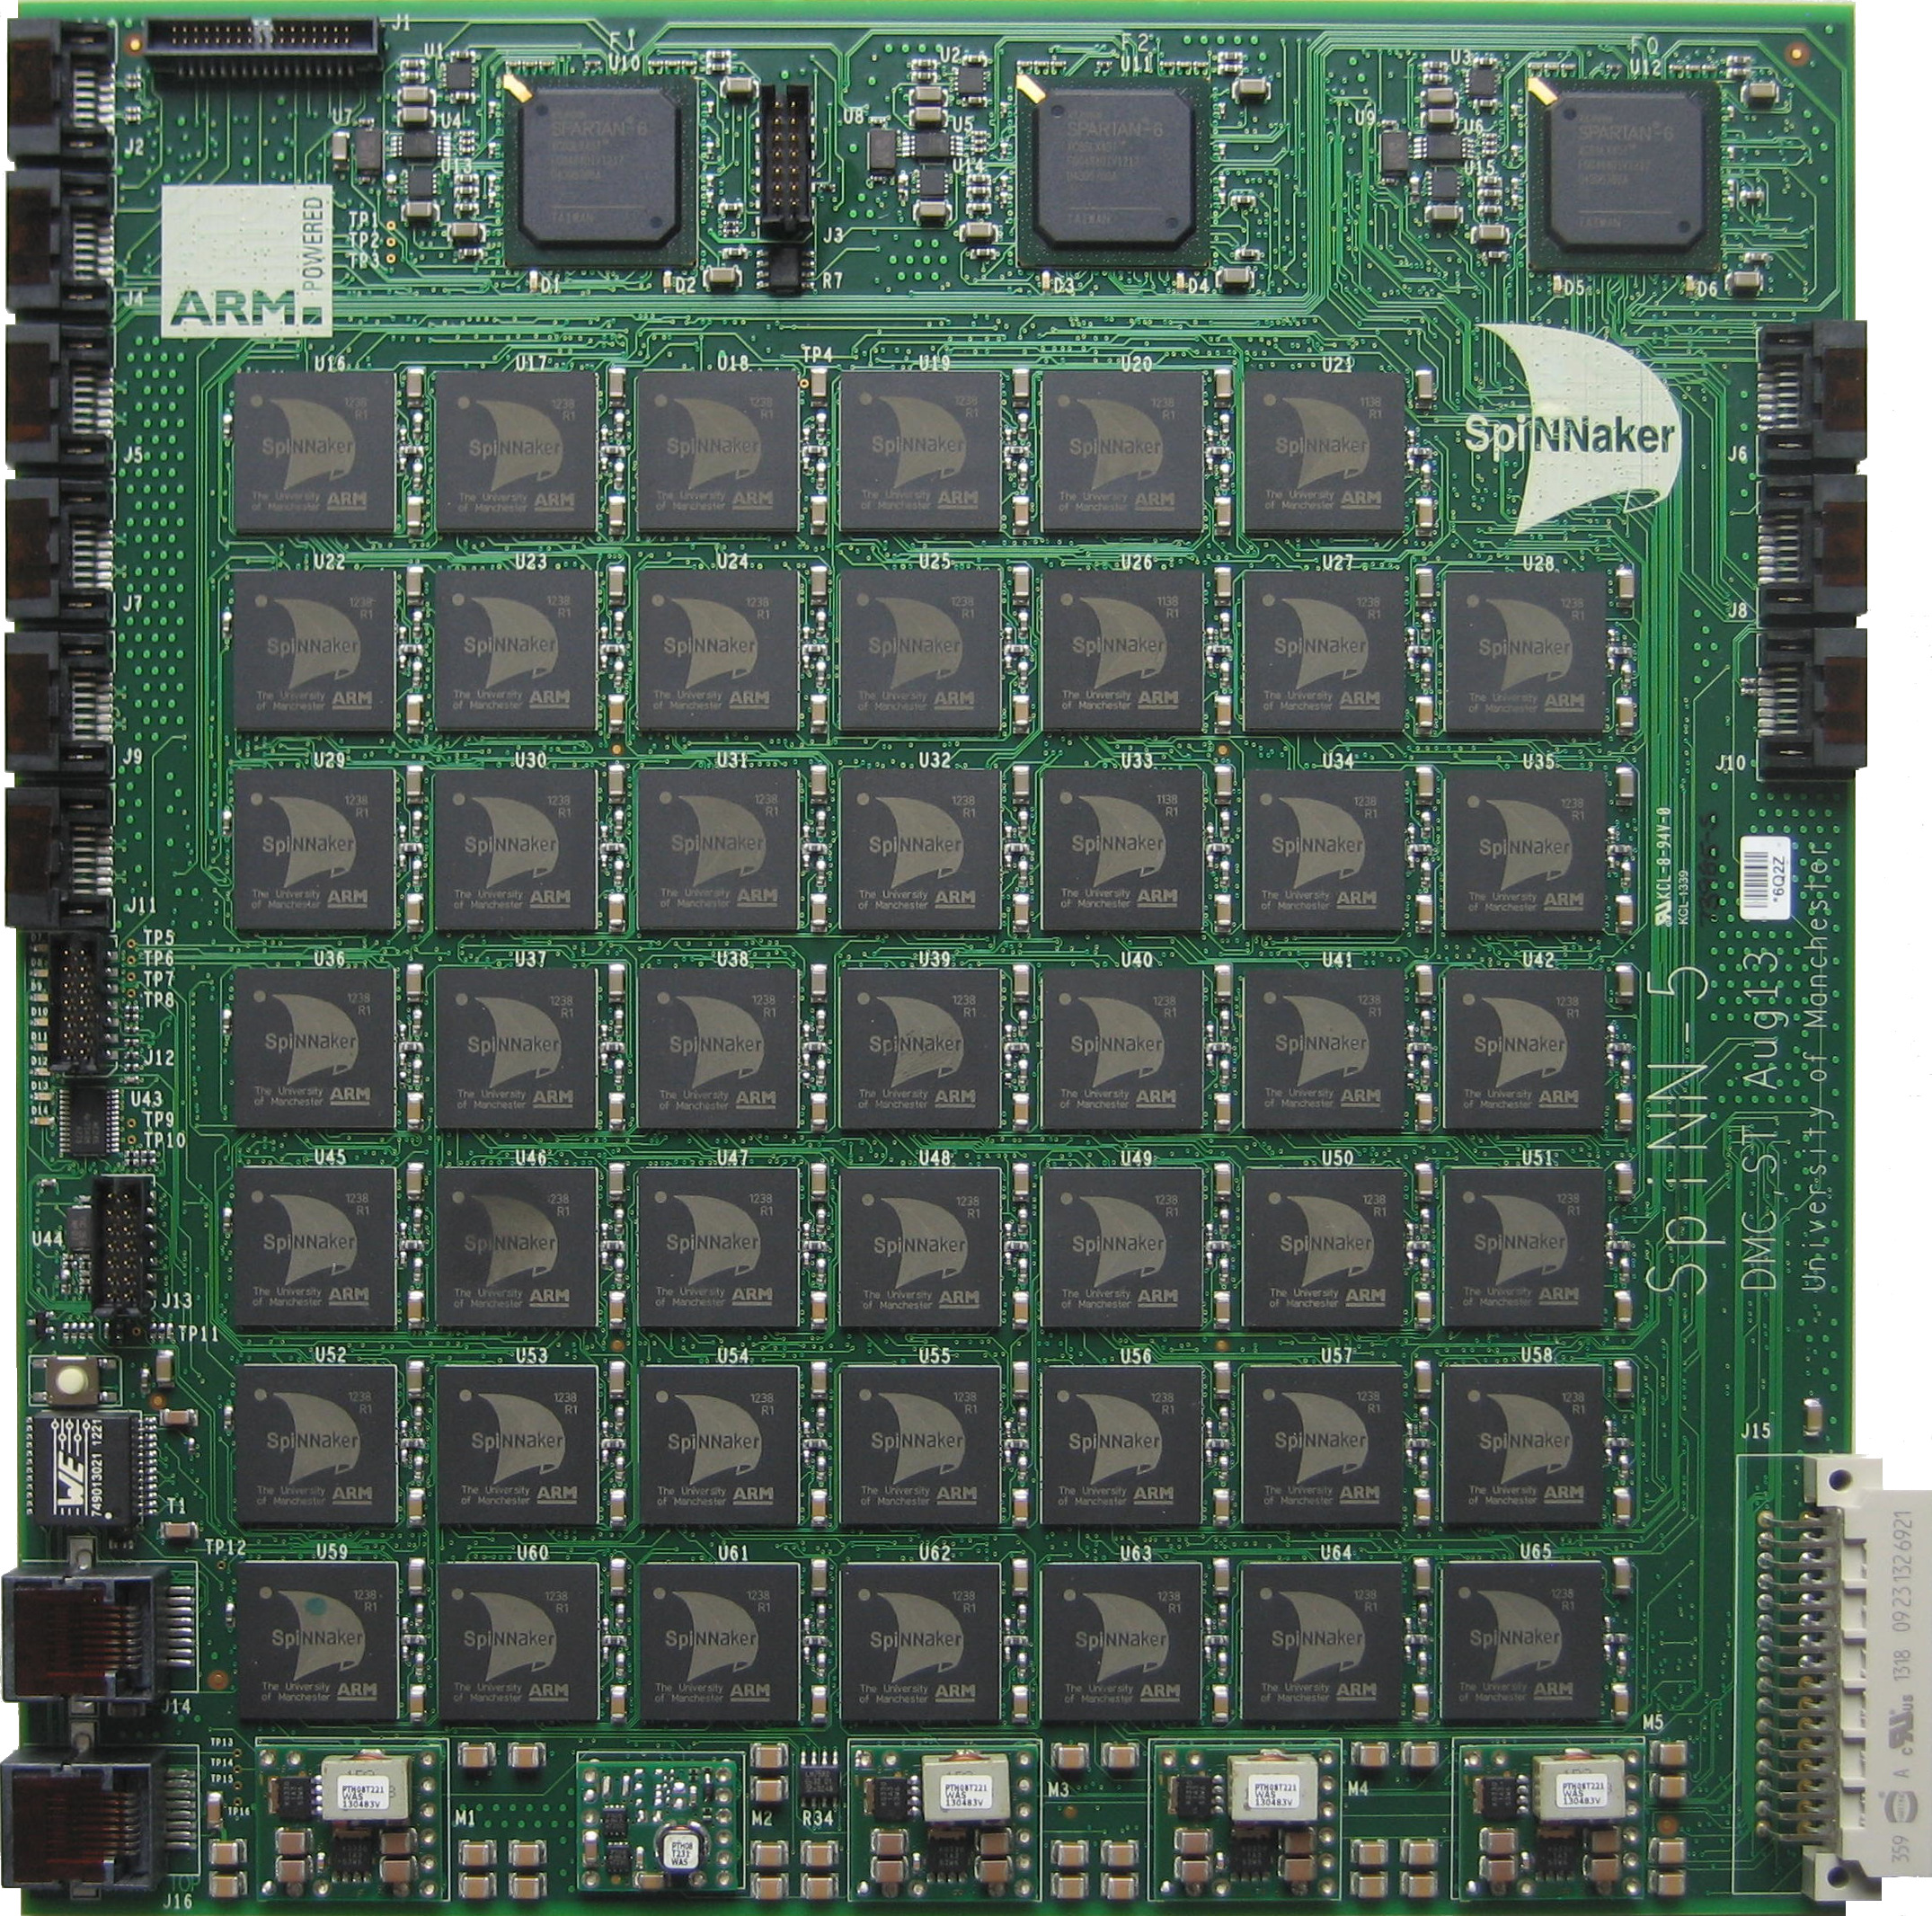
\includegraphics[width=.7\linewidth]
      {spinnakerBoard.jpg}
  \end{center}
\end{frame}
% }}}

% Prototype {{{
\section{Prototype}

\begin{frame}[fragile]
  \frametitle{User API}
  \setbeamercovered{invisible}

  \begin{figure} % {{{
  \begin{subfigure}[t]{.48\linewidth}
    {\tiny
  \begin{lstlisting}[language=Python]
import numpy as np
import tensorflow as tf

# generate random data set
X = np.random.rand(500, 10)

# Keras MLP
kmodel = tf.keras.models.Sequential()
kmodel.add(tf.keras.layers.Dense(
  50, activation="relu",
  input_shape=(10,)))
kmodel.add(tf.keras.layers.Dense(
  50, activation="softmax"))
kmodel.add(tf.keras.layers.Dense(
  300, activation="tanh"))
kmodel.add(tf.keras.layers.Dense(
  50, activation="sigmoid"))
kmodel.add(tf.keras.layers.Dense(25))

# predict labels from random data
# with random weights
p_ = kmodel.predict(X)
  \end{lstlisting}
}
  \end{subfigure}
  \begin{subfigure}[t]{.48\linewidth}
    {\tiny
  \begin{lstlisting}[language=Python]
from spiDNN import Model
from spiDNN.layers import Input, Dense

# equivalent model for SpiNNaker
model=Model()
model.add(Input(10))
model.add(Dense(50, activation="relu"))
model.add(Dense(50, activation="softmax"))
model.add(Dense(300, activation="tanh"))
model.add(Dense(50, activation="sigmoid"))
model.add(Dense(25))

# make sure both models have same parameters
model.set_weights(kmodel.get_weights())

p = model.predict(X)

# floating point discrepancies may occur
assert np.amax(np.absolute(p - p_)) < 1e-4
\end{lstlisting}
}
  \end{subfigure}
  \end{figure} % }}}
\end{frame}

\begin{frame}[fragile]
  \frametitle{Prototype Architecture}
  \setbeamercovered{invisible}

  {\tiny
  \begin{center} % {{{
    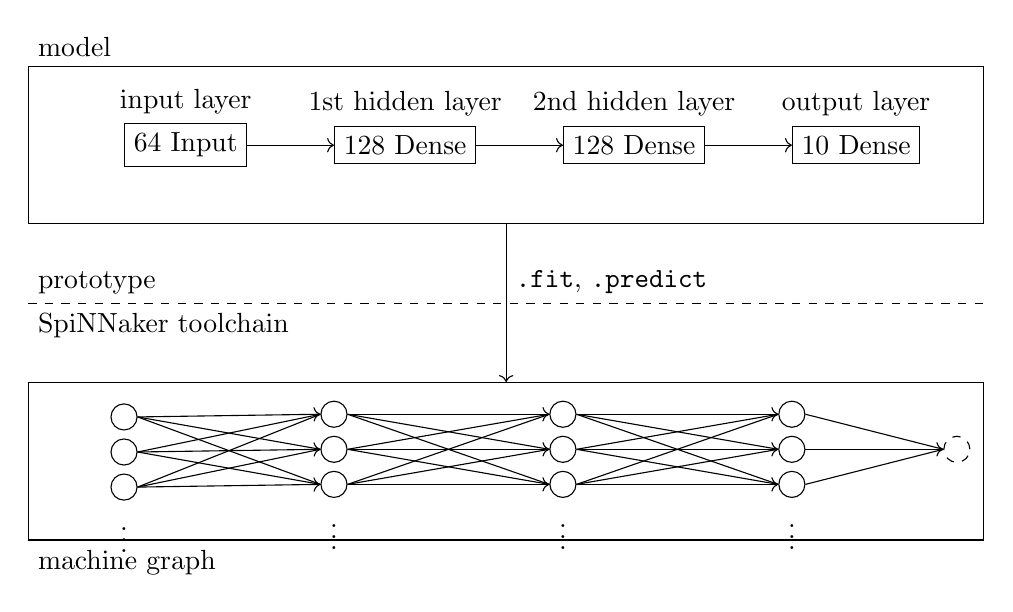
\begin{tikzpicture}[
      elem/.style={rectangle, draw},
      dot/.style={circle, draw},
      layer/.style={minimum width=1.2cm},
      container/.style={minimum width=\linewidth,
                         minimum height=2cm}
    ]
      \node[elem, container]
        at (0, 0) (model) {};
      \node[above right] at (model.north west) {model};

      \node[elem, layer, label=input layer]
        (layer_input) at ($(model.west) + (2, 0)$) {64 Input};
      \node[elem, layer, label=1st hidden layer, right=1.1 of layer_input]
        (layer_hidden1) {128 Dense};
      \node[elem, layer, label=2nd hidden layer, right=1.1 of layer_hidden1]
        (layer_hidden2) {128 Dense};
      \node[elem, layer, label=output layer, right=1.1 of layer_hidden2]
        (layer_output) {10 Dense};

      \draw[->] (layer_input) -- (layer_hidden1);
      \draw[->] (layer_hidden1) -- (layer_hidden2);
      \draw[->] (layer_hidden2) -- (layer_output);


      \draw[dashed] ($(model.south west) - (0, 1)$)
        node[above right] {prototype}
        node[below right] {SpiNNaker toolchain} --
        ($(model.south east) - (0, 1)$);

      \node[elem, container, below=2 of model] (machine_graph) {};
      \node[below right] at (machine_graph.south west)
        {machine graph};

      \node[dot, below=3 of layer_input.south west]
        (input0) {};
      \node[dot, below=.1 of input0]
        (input1) {};
      \node[dot, below=.1 of input1]
        (input2) {};
      \node[below=.001 of input2] {\vdots};

      \node[dot, below=3 of layer_hidden1.south west]
        (hidden00) {};
      \node[dot, below=.1 of hidden00]
        (hidden01) {};
      \node[dot, below=.1 of hidden01]
        (hidden02) {};
      \node[below=.001 of hidden02] {\vdots};

      \node[dot, below=3 of layer_hidden2.south west]
        (hidden10) {};
      \node[dot, below=.1 of hidden10]
        (hidden11) {};
      \node[dot, below=.1 of hidden11]
        (hidden12) {};
      \node[below=.001 of hidden12] {\vdots};

      \node[dot, below=3 of layer_output.south west]
        (output0) {};
      \node[dot, below=.1 of output0]
        (output1) {};
      \node[dot, below=.1 of output1]
        (output2) {};
      \node[below=.001 of output2] {\vdots};


      \node[dot, dashed, right=1.75 of output1] (lpg) {};


      \draw[->] (model) -- node[above right]
        {\texttt{.fit}, \texttt{.predict}} (machine_graph);

      \draw[->] (input0.east) -- (hidden00.west);
      \draw (input0.east) -- (hidden01.west);
      \draw (input0.east) -- (hidden02.west);

      \draw (input1.east) -- (hidden00.west);
      \draw[->] (input1.east) -- (hidden01.west);
      \draw (input1.east) -- (hidden02.west);

      \draw (input2.east) -- (hidden00.west);
      \draw (input2.east) -- (hidden01.west);
      \draw[->] (input2.east) -- (hidden02.west);

      \draw[->] (hidden00.east) -- (hidden10.west);
      \draw (hidden00.east) -- (hidden11.west);
      \draw (hidden00.east) -- (hidden12.west);

      \draw (hidden01.east) -- (hidden10.west);
      \draw[->] (hidden01.east) -- (hidden11.west);
      \draw (hidden01.east) -- (hidden12.west);

      \draw (hidden02.east) -- (hidden10.west);
      \draw (hidden02.east) -- (hidden11.west);
      \draw[->] (hidden02.east) -- (hidden12.west);

      \draw[->] (hidden10.east) -- (output0.west);
      \draw (hidden10.east) -- (output1.west);
      \draw (hidden10.east) -- (output2.west);

      \draw (hidden11.east) -- (output0.west);
      \draw[->] (hidden11.east) -- (output1.west);
      \draw (hidden11.east) -- (output2.west);

      \draw (hidden12.east) -- (output0.west);
      \draw (hidden12.east) -- (output1.west);
      \draw[->] (hidden12.east) -- (output2.west);

      \draw (output0.east) -- (lpg.west);
      \draw[->] (output1.east) -- (lpg.west);
      \draw (output2.east) -- (lpg.west);
    \end{tikzpicture}
  \end{center} % }}}
  }
\end{frame}

\begin{frame}[fragile]
  \frametitle{Features}
  \setbeamercovered{invisible}

  \begin{minipage}[t]{.48\textwidth}
    Supported Features
    \begin{itemize}
      \item Dense layers
      \item 1D convolutional layers
      \item (Flatten layers)
      \item Most common activation functions
      \item Most common loss functions
      \item SGD optimizer with constant learning rate
    \end{itemize}
  \end{minipage}
  \pause
  \begin{minipage}[t]{.48\textwidth}
    Missing Features
    \begin{itemize}
      \item 2D convolutional layers
      \item Pooling layers
      \item Shortcut connections \citep{he_et_al_2015}
      \item (Batch normalization)
    \end{itemize}
  \end{minipage}
\end{frame}
% }}}

% Problems {{{
\section{Problems}

\begin{frame}[fragile]
  \frametitle{Problems}
  \setbeamercovered{invisible}

  \begin{itemize}[<+->]
    \item TIME!
    \item Dropped packets
    \item Convolutional layer as neurons is a complex abstraction
  \end{itemize}
\end{frame}
% }}}

% Next steps {{{
\section{Next Steps}

\begin{frame}[fragile]
  \frametitle{Overcoming Dropped Packets in the Future}
  \setbeamercovered{invisible}

  SpiNNaker APIs we were not able to try:
  \pause
  \begin{itemize}[<+->]
    \item Application graph instead of machine graph (less packets
      sent)
    \item P2P communications instead of multicast packets
    \item Time-division multiple access (TDMA) system (sends packets
      at the right time to avoid dropping them)
  \end{itemize}
\end{frame}

\begin{frame}[fragile]
  \frametitle{Overcoming Dropped Packets in the Future}
  \setbeamercovered{invisible}

  Better domain decomposition:
  {\tiny
\begin{figure} % {{{
    \begin{center}
    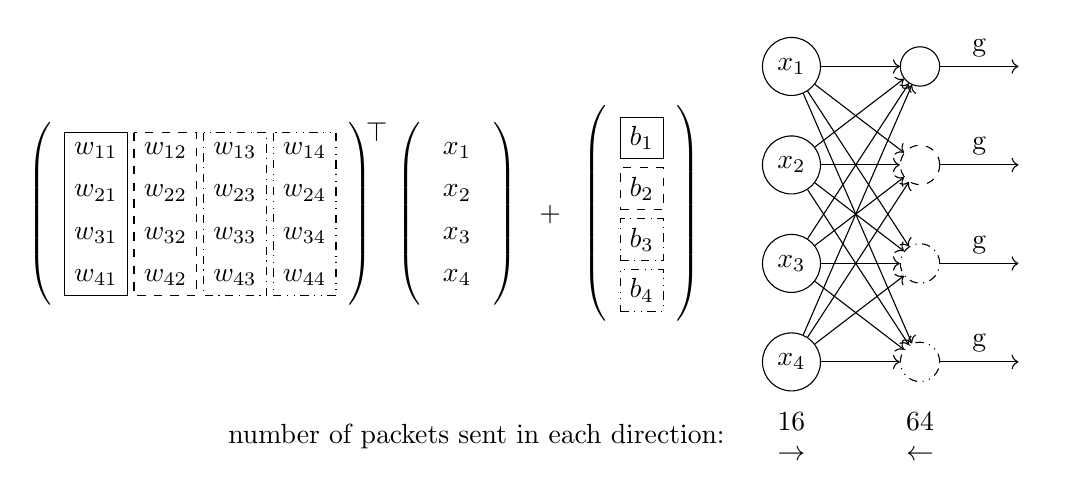
\begin{tikzpicture}[dot/.style={circle,draw, minimum size=.5cm}]
      \matrix[left delimiter=(, right delimiter=), column sep=.1cm, row sep=.1cm] (w) {
        \node (w_11) {$w_{11}$}; & \node (w_12) {$w_{12}$}; & \node (w_13) {$w_{13}$}; & \node (w_14) {$w_{14}$}; \\
        \node (w_21) {$w_{21}$}; & \node (w_22) {$w_{22}$}; & \node (w_23) {$w_{23}$}; & \node (w_24) {$w_{24}$}; \\
        \node (w_31) {$w_{31}$}; & \node (w_32) {$w_{32}$}; & \node (w_33) {$w_{33}$}; & \node (w_34) {$w_{34}$}; \\
        \node (w_41) {$w_{41}$}; & \node (w_42) {$w_{42}$}; & \node (w_43) {$w_{43}$}; & \node (w_44) {$w_{44}$}; \\
      };
      \node at ($(w.north east) + (.4,-.1)$) {$\top$};
      \matrix[right=1 of w, row sep=.1cm, left delimiter=(, right delimiter=)] (x) {
        \node{$x_1$}; \\
        \node{$x_2$}; \\
        \node{$x_3$}; \\
        \node{$x_4$}; \\
      };
      \node[right=.5 of x] (add) {+};
      \matrix[right=.5 of add, row sep=.1cm, left delimiter=(, right delimiter=)] (b) {
        \node[draw]{$b_1$}; \\
        \node[draw, dashed]{$b_2$}; \\
        \node[draw, dash dot]{$b_3$}; \\
        \node[draw, dash dot dot]{$b_4$}; \\
      };

      \matrix[right = 1 of b, column sep=1cm, row sep=.5cm] {
        \node[dot] (x_1) {$x_1$}; & \node[dot] (n_1) {}; & \node (o_1) {}; \\
        \node[dot] (x_2) {$x_2$}; & \node[dot, dashed] (n_2) {}; & \node (o_2) {}; \\
        \node[dot] (x_3) {$x_3$}; & \node[dot, dash dot] (n_3) {}; & \node (o_3) {}; \\
        \node[dot] (x_4) {$x_4$}; & \node[dot, dash dot dot] (n_4) {}; & \node (o_4) {}; \\
      };

      \node[below=1 of x_4.center, label=16] (packets) {$\rightarrow$};
      \node[below=1 of n_4.center, label=64] {$\leftarrow$};
        \node at ($(packets.north) - (4,-.05)$) {number of packets sent in each direction:};

      \draw[->] (x_1) -- (n_1);
      \draw[->] (x_1) -- (n_2);
      \draw[->] (x_1) -- (n_3);
      \draw[->] (x_1) -- (n_4);

      \draw[->] (x_2) -- (n_1);
      \draw[->] (x_2) -- (n_2);
      \draw[->] (x_2) -- (n_3);
      \draw[->] (x_2) -- (n_4);

      \draw[->] (x_3) -- (n_1);
      \draw[->] (x_3) -- (n_2);
      \draw[->] (x_3) -- (n_3);
      \draw[->] (x_3) -- (n_4);

      \draw[->] (x_4) -- (n_1);
      \draw[->] (x_4) -- (n_2);
      \draw[->] (x_4) -- (n_3);
      \draw[->] (x_4) -- (n_4);

      \draw[->] (n_1) -- node[above]{g} (o_1);
      \draw[->] (n_2) -- node[above]{g} (o_2);
      \draw[->] (n_3) -- node[above]{g} (o_3);
      \draw[->] (n_4) -- node[above]{g} (o_4);

      \draw (w_11.north west) |- (w_41.south west) -| (w_11.north east) -- cycle;
      \draw[dashed] (w_12.north west) |- (w_42.south west) -| (w_12.north east) -- cycle;
      \draw[dash dot] (w_13.north west) |- (w_43.south west) -| (w_13.north east) -- cycle;
      \draw[dash dot dot] (w_14.north west) |- (w_44.south west) -| (w_14.north east) -- cycle;
    \end{tikzpicture}
    \end{center}
    \caption{How the computational graph of a dense layer is
      decomposed into neurons (implemented by the prototype).}
  \end{figure} % }}}
  }
\end{frame}

\begin{frame}[fragile]
  \frametitle{Overcoming Dropped Packets in the Future}
  \setbeamercovered{invisible}

  Better domain decomposition:
  {\tiny
\begin{figure} % {{{
    \begin{center}
    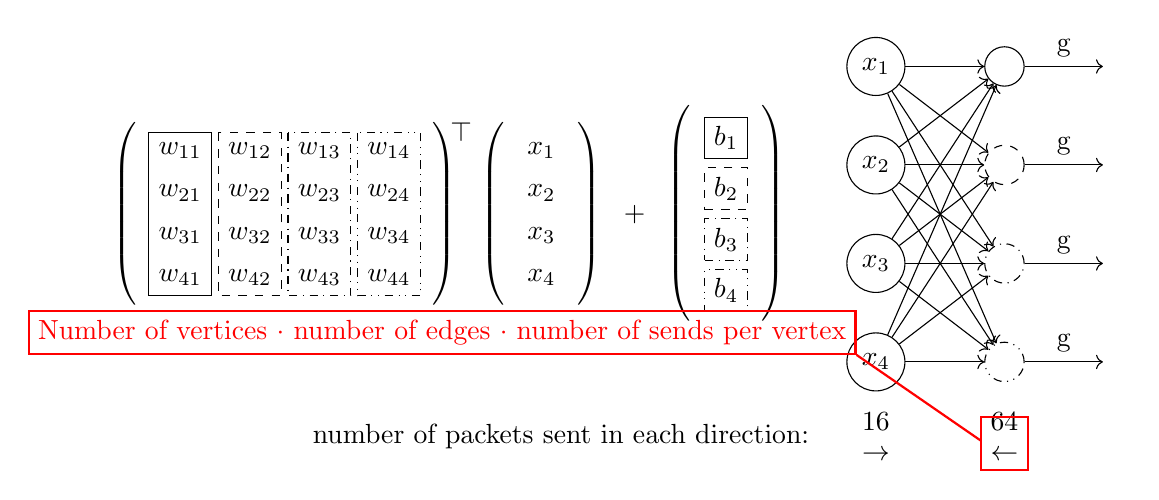
\begin{tikzpicture}[dot/.style={circle,draw, minimum size=.5cm}]
      \matrix[left delimiter=(, right delimiter=), column sep=.1cm, row sep=.1cm] (w) {
        \node (w_11) {$w_{11}$}; & \node (w_12) {$w_{12}$}; & \node (w_13) {$w_{13}$}; & \node (w_14) {$w_{14}$}; \\
        \node (w_21) {$w_{21}$}; & \node (w_22) {$w_{22}$}; & \node (w_23) {$w_{23}$}; & \node (w_24) {$w_{24}$}; \\
        \node (w_31) {$w_{31}$}; & \node (w_32) {$w_{32}$}; & \node (w_33) {$w_{33}$}; & \node (w_34) {$w_{34}$}; \\
        \node (w_41) {$w_{41}$}; & \node (w_42) {$w_{42}$}; & \node (w_43) {$w_{43}$}; & \node (w_44) {$w_{44}$}; \\
      };
      \node at ($(w.north east) + (.4,-.1)$) {$\top$};
      \matrix[right=1 of w, row sep=.1cm, left delimiter=(, right delimiter=)] (x) {
        \node{$x_1$}; \\
        \node{$x_2$}; \\
        \node{$x_3$}; \\
        \node{$x_4$}; \\
      };
      \node[right=.5 of x] (add) {+};
      \matrix[right=.5 of add, row sep=.1cm, left delimiter=(, right delimiter=)] (b) {
        \node[draw]{$b_1$}; \\
        \node[draw, dashed]{$b_2$}; \\
        \node[draw, dash dot]{$b_3$}; \\
        \node[draw, dash dot dot]{$b_4$}; \\
      };

      \matrix[right = 1 of b, column sep=1cm, row sep=.5cm] {
        \node[dot] (x_1) {$x_1$}; & \node[dot] (n_1) {}; & \node (o_1) {}; \\
        \node[dot] (x_2) {$x_2$}; & \node[dot, dashed] (n_2) {}; & \node (o_2) {}; \\
        \node[dot] (x_3) {$x_3$}; & \node[dot, dash dot] (n_3) {}; & \node (o_3) {}; \\
        \node[dot] (x_4) {$x_4$}; & \node[dot, dash dot dot] (n_4) {}; & \node (o_4) {}; \\
      };

      \node[below=1 of x_4.center, label=16] (packets) {$\rightarrow$};
      \node[below=1 of n_4.center, label=64] (lbl) {$\leftarrow$};
        \node at ($(packets.north) - (4,-.05)$) {number of packets sent in each direction:};

      \draw[thick, red] (lbl.south west) rectangle ($(lbl.north east) + (0,.3)$);

      \node[draw, thick, red] at (2, -1.5) (txt) {Number of vertices $\cdot$ number of edges
        $\cdot$ number of sends per vertex};

      \draw[thick, red] (txt.south east) -- (lbl.north west);

      \draw[->] (x_1) -- (n_1);
      \draw[->] (x_1) -- (n_2);
      \draw[->] (x_1) -- (n_3);
      \draw[->] (x_1) -- (n_4);

      \draw[->] (x_2) -- (n_1);
      \draw[->] (x_2) -- (n_2);
      \draw[->] (x_2) -- (n_3);
      \draw[->] (x_2) -- (n_4);

      \draw[->] (x_3) -- (n_1);
      \draw[->] (x_3) -- (n_2);
      \draw[->] (x_3) -- (n_3);
      \draw[->] (x_3) -- (n_4);

      \draw[->] (x_4) -- (n_1);
      \draw[->] (x_4) -- (n_2);
      \draw[->] (x_4) -- (n_3);
      \draw[->] (x_4) -- (n_4);

      \draw[->] (n_1) -- node[above]{g} (o_1);
      \draw[->] (n_2) -- node[above]{g} (o_2);
      \draw[->] (n_3) -- node[above]{g} (o_3);
      \draw[->] (n_4) -- node[above]{g} (o_4);

      \draw (w_11.north west) |- (w_41.south west) -| (w_11.north east) -- cycle;
      \draw[dashed] (w_12.north west) |- (w_42.south west) -| (w_12.north east) -- cycle;
      \draw[dash dot] (w_13.north west) |- (w_43.south west) -| (w_13.north east) -- cycle;
      \draw[dash dot dot] (w_14.north west) |- (w_44.south west) -| (w_14.north east) -- cycle;
    \end{tikzpicture}
    \end{center}
    \caption{How the computational graph of a dense layer is
      decomposed into neurons (implemented by the prototype).}
  \end{figure} % }}}
  }
\end{frame}

\begin{frame}[fragile]
  \frametitle{Overcoming Dropped Packets in the Future}
  \setbeamercovered{invisible}

  Better domain decomposition:
  {\tiny
  \begin{figure} % {{{
    \begin{center}
    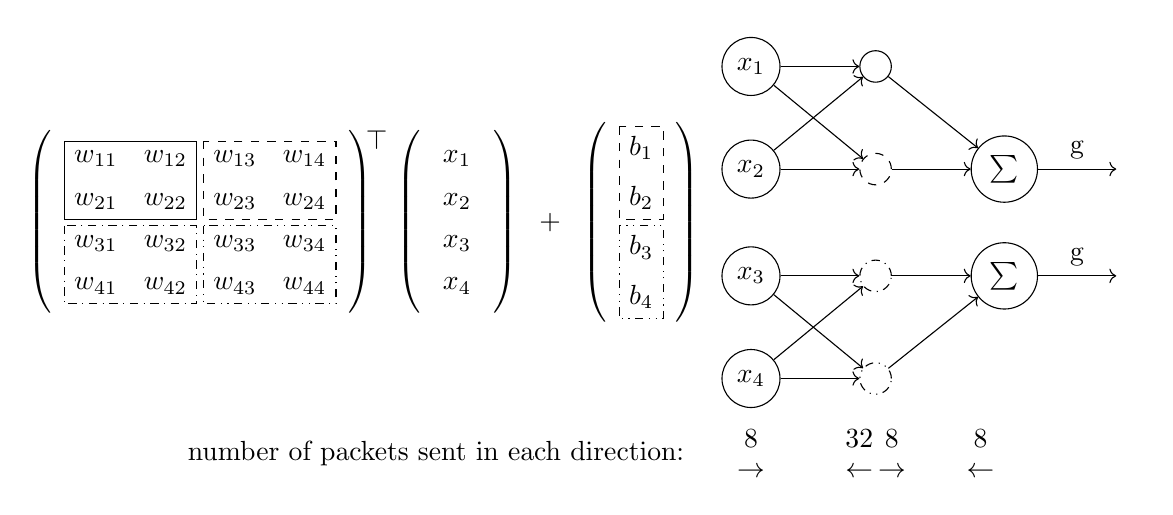
\begin{tikzpicture}[dot/.style={circle,draw, minimum size=.4cm}]
      \matrix[left delimiter=(, right delimiter=), column sep=.1cm, row sep=.1cm] (w) {
        \node (w_11) {$w_{11}$}; & \node (w_12) {$w_{12}$}; & \node (w_13) {$w_{13}$}; & \node (w_14) {$w_{14}$}; \\
        \node (w_21) {$w_{21}$}; & \node (w_22) {$w_{22}$}; & \node (w_23) {$w_{23}$}; & \node (w_24) {$w_{24}$}; \\
        \node (w_31) {$w_{31}$}; & \node (w_32) {$w_{32}$}; & \node (w_33) {$w_{33}$}; & \node (w_34) {$w_{34}$}; \\
        \node (w_41) {$w_{41}$}; & \node (w_42) {$w_{42}$}; & \node (w_43) {$w_{43}$}; & \node (w_44) {$w_{44}$}; \\
      };
      \node at ($(w.north east) + (.4,-.1)$) {$\top$};
      \matrix[right=1 of w, row sep=.1cm, left delimiter=(, right delimiter=)] (x) {
        \node{$x_1$}; \\
        \node{$x_2$}; \\
        \node{$x_3$}; \\
        \node{$x_4$}; \\
      };
      \node[right=.5 of x] (add) {+};
      \matrix[right=.5 of add, row sep=.1cm, left delimiter=(, right delimiter=)] (b) {
        \node (b_1) {$b_1$}; \\
        \node (b_2) {$b_2$}; \\
        \node (b_3) {$b_3$}; \\
        \node (b_4) {$b_4$}; \\
      };

      \matrix[right = .5 of b, column sep=1cm, row sep=.5cm] {
        \node[dot] (x_1) {$x_1$}; & \node[dot] (n_1) {}; & \node (o_1) {}; & \node (oo_1) {}; \\
        \node[dot] (x_2) {$x_2$}; & \node[dot, dashed] (n_2) {}; & \node[dot] (o_2) {$\sum$}; & \node (oo_2) {}; \\
        \node[dot] (x_3) {$x_3$}; & \node[dot, dash dot] (n_3) {}; & \node[dot] (o_3) {$\sum$}; & \node (oo_3) {}; \\
        \node[dot] (x_4) {$x_4$}; & \node[dot, dash dot dot] (n_4) {}; & \node (o_4) {}; & \node (oo_4) {}; \\
      };

      \node[below=1 of x_4.center, label=8] (packets) {$\rightarrow$};
      \node[below=1 of n_4.west, label=32] {$\leftarrow$};
      \node[below=1 of n_4.east, label=8] {$\rightarrow$};
      \node[below=1 of o_4.center, label=8] {$\leftarrow$};
        \node at ($(packets.north) - (4,-.05)$) {number of packets sent in each direction:};

      \draw[->] (x_1) -- (n_1);
      \draw[->] (x_1) -- (n_2);

      \draw[->] (x_2) -- (n_1);
      \draw[->] (x_2) -- (n_2);

      \draw[->] (x_3) -- (n_3);
      \draw[->] (x_3) -- (n_4);

      \draw[->] (x_4) -- (n_3);
      \draw[->] (x_4) -- (n_4);

      \draw[->] (n_1) -- (o_2);
      \draw[->] (n_2) -- (o_2);
      \draw[->] (n_3) -- (o_3);
      \draw[->] (n_4) -- (o_3);

      \draw[->] (o_2) -- node[above]{g} (oo_2);
      \draw[->] (o_3) -- node[above]{g} (oo_3);

      \draw (w_11.north west) |- (w_21.south west) -| (w_12.north east) -- cycle;
      \draw[dashed] (w_13.north west) |- (w_23.south west) -| (w_14.north east) -- cycle;
      \draw[dash dot] (w_31.north west) |- (w_41.south west) -| (w_32.north east) -- cycle;
      \draw[dash dot dot] (w_33.north west) |- (w_43.south west) -| (w_34.north east) -- cycle;

      \draw[dashed] (b_1.north west) |- (b_2.south west) -| (b_1.north east) -- cycle;
      \draw[dash dot dot] (b_3.north west) |- (b_4.south west) -| (b_3.north east) -- cycle;
    \end{tikzpicture}
    \end{center}
    \caption{How the computational graph of a dense layer could
      be decomposed in order to reduce the peak and overall number of
      packets by sparsifying the graph.}
    \end{figure} % }}}
  }
\end{frame}

% }}}

% References {{{
\begin{frame}
  \frametitle{References}
  \bibliography{literature.bib}
\end{frame}
% }}}

\end{document}
